In this appendix we explore in more detail the mixing behavior presented in the main body via additional metrics, and considering a wider range of models.

\subsection{Input Independent Metrics}

As our work is concerned largely with how the functionality of layers change throughout depth as the residual stream is iteratively updated, our primary concern is with \emph{input-dependent} measures of stages of inference: ColSum concentration as presented in the main text of the paper is one such input-dependent metric, and the later sections of this appendix will introduce and present results for a wider range of such metrics.

However, to bridge the gap between our work and that of \citet{lad2024remarkable}, we also present results for the fraction of \emph{prediction and suppression} neurons \citep{gurnee2024universal} in successive layers of both feedforward and looped Transformers. We highlight however that \emph{these are unable to change with successive recurrences}, and are thus secondary to our focus. \Cref{fig:feedforward_prediction_neurons} presents results for a selection of feedforward models used throughout the paper, and \Cref{fig:looped_prediction_neurons} presents results for a selection of looped models used throughout the paper. Similar to our results elsewhere, we find that the looped model stages of inference in these metrics tend to mirror those of feedforward models.

\begin{figure*}[ht]
    \centering    
    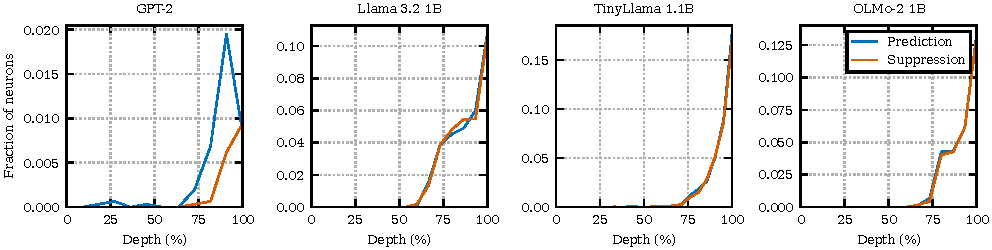
\includegraphics{figures/prediction_neurons/feedforward.pdf}
    \caption{\textbf{Fraction of prediction and suppression neurons in a selection of feedforward models used throughout the paper}.}
    \label{fig:feedforward_prediction_neurons}
\end{figure*}

\begin{figure*}[ht]
    \centering    
    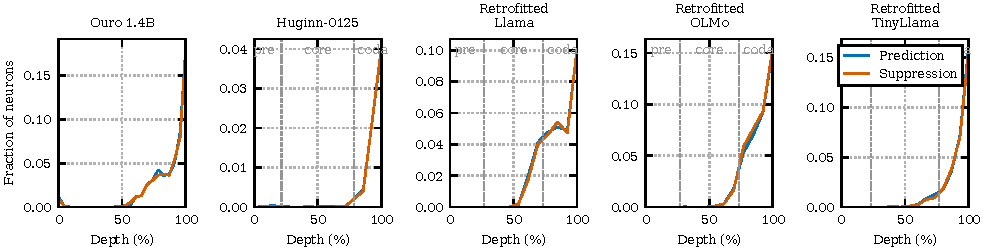
\includegraphics{figures/prediction_neurons/looped.pdf}
    \caption{\textbf{Fraction of prediction and suppression neurons in a selection of looped models used throughout the paper}.}
    \label{fig:looped_prediction_neurons}
\end{figure*}

\subsection{Input Dependent Metrics}\label{appen:input_dependent_soi_metrics}

One well-studied phenomenon by which Transformers drastically \emph{reduce} the mixing in given layer is that of the \emph{attention sink} \citep{xiao2023efficient,barbero2025llms}, whereby the layer focuses the majority of the attention ``weight'' onto the first token in the sequence; often this is the BOS (beginning of sequence) token, and thus completely uninformative. To measure this behavior, we adopt the \textbf{attention sink score} and \textbf{sink rate} of \citet{gu2024attention}: for token position $k$ and sequence length $T$, the sink score at layer $\ell$ and head $h$ is defined as:
\begin{equation}
    \text{sink-score}_k^{(\ell,h)} = \frac{1}{T}\sum_{t=0}^{T-1}A_{tk}^{(\ell,h)},
\end{equation}
where $A_{tk}^{(\ell,h)}$ corresponds to the realized attention matrix of \Cref{eq:attn_in_a} at layer $\ell$, head $h$. The sink rate is then defined as the fraction of heads for which the sink score lies above a certain threshold:
\begin{equation}
    \text{sink-rate}^{(\ell)}_k = \frac{1}{H}\sum_{h=1}^H\mathbb{I}\!\left(\text{sink-score}_k^{(\ell,h)}\geq \tau\right),
\end{equation}
where following related work we define a threshold of $\tau=0.3$, and $\mathbb{I}$ denotes the indicator function.

We also adopt the \emph{Mixing score} of \citet{queipo2025attention}: for sequence length $T$, layer $\ell$ and head $h$ this is defined as the average row entropy of the attention matrices:
\begin{equation}
    \text{mixing-score}^{(\ell,h)} = \frac{1}{T} \sum_{i=1}^T H(A_{i, :}^{(\ell, h)}).
\end{equation}

Following \citet{skean2025layer,queipo2025attention} we additionally measure the compression of the residual stream $\mX$ via the matrix-based entropy $H(\mX)$.

In the plots that follow we average sink rates, Mixing scores and ColSum concentrations over all the heads in a layer, and over all input sequences. Residual entropy is averaged over all input sequences.

\FloatBarrier
\subsection{Cyclic Stages of Inference}\label{appen:cyclic_soi}

Supplementing the cyclic recurrence in realized depth for retrofitted Llama in \Cref{fig:stages_of_inference_cyclic_and_similar}, we additionally overlay cycles in realized depth for \ouro{} and \raven{} in \Cref{fig:stages_of_inference_cyclic_extended}, where all models are run for 8 recurrences. This demonstrates that for \textbf{sink rates and mixing scores}, the cyclic behavior and lack of significant depth-wise changes hold both for the other investigated models, and the additional stages of inference metrics.

The results for residual entropy are more nuanced: while the results for \raven{} and the retrofitted models show broadly the same behavior as the attention-based metrics, \ouro{} demonstrates different behavior. As shown in \Cref{fig:ouro_recurrent_block_stages}, the residual entropies both change significantly with successive recurrences and do not closely follow the feedforward behavior. We believe that the divergence from feedforward behavior may derive from the norm structure of this model: the residual stream is normalised after each recurrent block, as visualised in \Cref{fig:residual_norm_comparison}, thus periodically shutting down massive activations. This is not the case for the retrofitted series of models, which lack this norm and show much closer alignment with feedforward stages of inference.

\begin{figure*}[ht]
    \centering    
    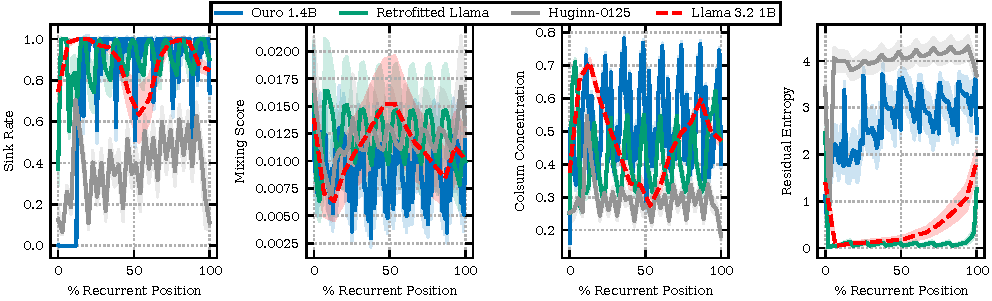
\includegraphics{figures/stages_of_inference/cyclic_behaviour_extended.pdf}
    \caption{\textbf{Stages of inference for a selection of Looped transformers, all using 8 recurrences}: \raven{} \citep{geiping2025scaling}, Ouro 1.4B \citep{zhu2025scaling} and Llama with retrofitted recurrences \citep{mcleish2025teaching}. Note \raven{} and Retrofitted Llama have prelude and coda layers too: each 2 layers in \raven{} and each 4 in Retrofitted Llama.}
    \label{fig:stages_of_inference_cyclic_extended}
\end{figure*}

For completeness, we plot these stages of inference for all other models referenced in the paper. See \Cref{fig:ouro_recurrent_block_stages} (Ouro 1.4B), \Cref{fig:raven_recurrent_block_stages} (\raven{}), \Cref{fig:retrofitted_llama_recurrent_block_stages,fig:retrofitted_olmo_recurrent_block_stages,fig:retrofitted_tinyllama_recurrent_block_stages} (retrofitted Llama, OLMo and TinyLlama).

\begin{figure}
    \centering    
    
\includegraphics{figures/stages_of_inference/recurrent/Ouro_1.4B_4_steps.pdf}
    \caption{\textbf{Stages of inference for each recurrent loop in Ouro 1.4B.} The close overlap with feedforward stages of inference is a particularly striking result as this model is trained from scratch with recurrence.}
    \label{fig:ouro_recurrent_block_stages}
\end{figure}

\begin{figure}
    \centering    
    
\includegraphics{figures/stages_of_inference/recurrent/Huginn-0125.pdf}
    \caption{\textbf{Stages of inference for each recurrent loop in \raven{}.} This represents a negative result: stages of inference do not occur. We discuss possible causes for this in the main text.}
    \label{fig:raven_recurrent_block_stages}
\end{figure}

\begin{figure}
    \centering    
    
\includegraphics{figures/stages_of_inference/recurrent/Retrofitted_Llama.pdf}
    \caption{\textbf{Stages of inference for each recurrent loop in the retrofitted Llama model \citep{mcleish2025teaching}.} Each block demonstrates very similar stages of inference to Llama, the base model from which pretrained layers are taken.}
    \label{fig:retrofitted_llama_recurrent_block_stages}
\end{figure}

\begin{figure}
    \centering    
    
\includegraphics{figures/stages_of_inference/recurrent/Retrofitted_OLMo.pdf}
    \caption{\textbf{Stages of inference for each recurrent loop in the retrofitted OLMo model \citep{mcleish2025teaching}.} Similarly, each block demonstrates very similar stages of inference to OLMo, the base model from which pretrained layers are taken.}
    \label{fig:retrofitted_olmo_recurrent_block_stages}
\end{figure}

\begin{figure}
    \centering    
    
\includegraphics{figures/stages_of_inference/recurrent/Retrofitted_TinyLlama.pdf}
    \caption{\textbf{Stages of inference for each recurrent loop in the retrofitted TinyLlama model \citep{mcleish2025teaching}.} Similarly, each block demonstrates very similar stages of inference to TinyLlama, the base model from which pretrained layers are taken.}
    \label{fig:retrofitted_tinyllama_recurrent_block_stages}
\end{figure}

We plot stages of inference for \ouro{} 2.6B in \Cref{fig:ouro_2_recurrent_block_stages}. This model is interesting due to the training regime followed by \citet{zhu2025scaling}, which ``upcycles'' a 48 layer model from the 24 layer 1.4B parameter model. As a consequence, the first and second half of each recurrent block each independently align with the Llama feedforward stages of inference.

\begin{figure}
    \centering    
    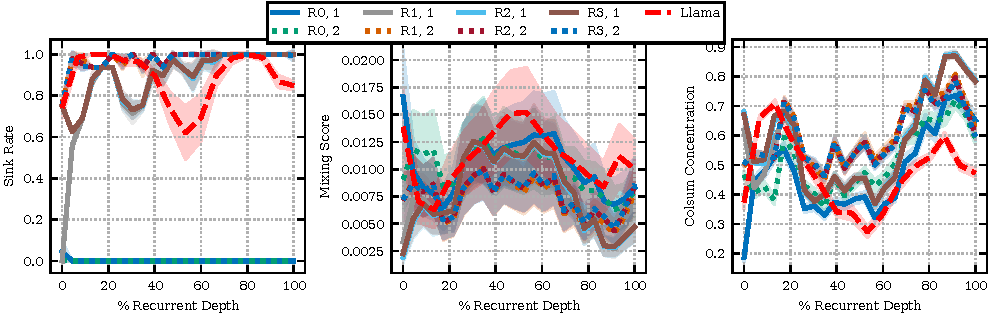
\includegraphics{figures/stages_of_inference/recurrent/Ouro_2.6B.pdf}
    \caption{\textbf{Stages of inference for each recurrent loop in Ouro 2.6B.} For this model we separate out the first and second half of the recurrent block and overlay them, demonstrating that both halves have close alignment with the Llama feedforward stages of inference. We suggest that this likely arises due to the training regime of \citet{zhu2025scaling}, which first trains a single 24 layer 1.4B parameter model, and then ``upcycles'' this into a 48 layer 2.6B parameter model by duplicating these layers, consequently duplicating the stages of inference as well.}
    \label{fig:ouro_2_recurrent_block_stages}
\end{figure}

In \Cref{sec:stages_of_inference} we suggested that the lack of stages of inference in \raven{} is likely due to the normalization of the residual stream resulting in massive activations being unable to form. Here we further support this suggestion by ablating the massive activations from the \rllama{} model (which \emph{does} display stages of inference) via zeroing the output of the MLP in the second layer, which is responsible for its massive activations. In this setting, visualized in \Cref{fig:ablation_rllama}, we see that the model no longer exhibits stages of inference comparable to the feedforward model, suggesting that the presence of massive activations is required for stages of inference to emerge in looped models.

\begin{figure}
    \centering    
    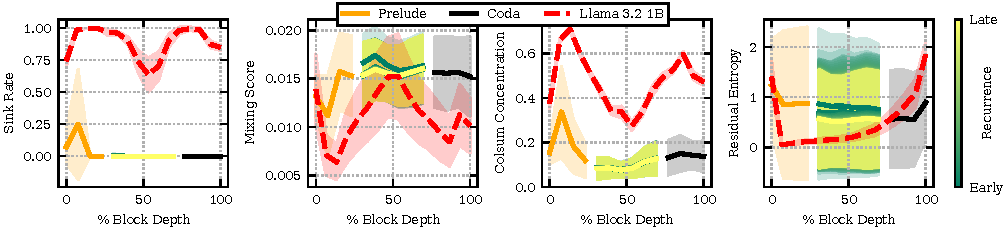
\includegraphics{figures/stages_of_inference/ablation_retrofitted_llama_bos_mlp.pdf}
    \caption{\textbf{Stages of inference for each recurrent loop in \rllama{} for which the massive activations have been ablated.} }
    \label{fig:ablation_rllama}
\end{figure}

\FloatBarrier
\subsection{Non-Reasoning Stages of Inference}\label{appen:hellaswag_soi}

Throughout the rest of the paper, experiments are conducted on the GSM8k dataset. In this appendix we verify that the stages of inference we observe are not specific to this dataset, and also occur in a non-reasoning setting, for which we use the HellaSwag dataset \citep{zellers2019hellaswag}. We follow an identical experimental setup to the GSM8k experiments, running inference on 256 random examples from the test split.

We present results in \Cref{fig:ouro_recurrent_block_stages_hellaswag} (Ouro 1.4B), \Cref{fig:raven_recurrent_block_stages_hellaswag} (\raven{}), \Cref{fig:retrofitted_llama_recurrent_block_stages_hellaswag,fig:retrofitted_olmo_recurrent_block_stages_hellaswag,fig:retrofitted_tinyllama_recurrent_block_stages_hellaswag} (retrofitted Llama, OLMo and TinyLlama). These show very few deviations from the GSM8k results, and the conclusions throughout the rest of the paper hold. However, we highlight the following small differences:
\begin{itemize}
    \item Across the board, sink rates tend to be higher in the HellaSwag setting.
    \item In \rolmo{}, ColSum concentration appears to be slightly higher in the HellaSwag setting.
\end{itemize}


\begin{figure}[ht]
    \centering    
    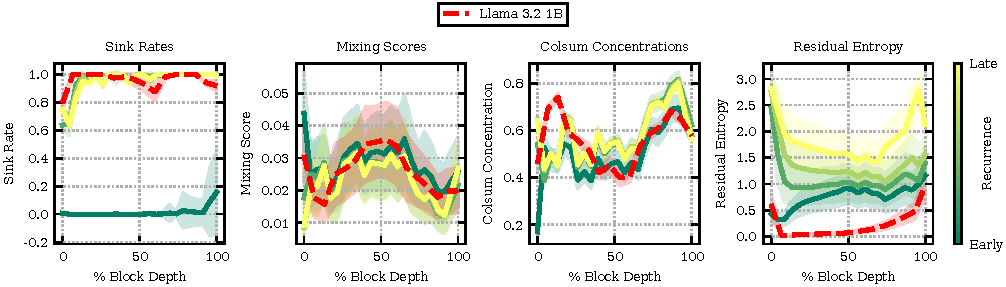
\includegraphics{figures/hellaswag/stages_of_inference/recurrent/Ouro_1.4B_4_steps.pdf}
    \caption{\textbf{Stages of inference for each recurrent loop in Ouro 1.4B, run on the HellaSwag dataset.}}
    \label{fig:ouro_recurrent_block_stages_hellaswag}
\end{figure}

\begin{figure}[ht]
    \centering    
    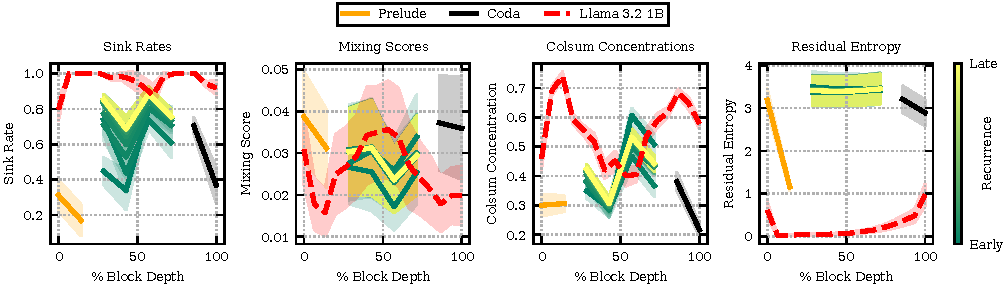
\includegraphics{figures/hellaswag/stages_of_inference/recurrent/Huginn-0125.pdf}
    \caption{\textbf{Stages of inference for each recurrent loop in \raven{}, run on the HellaSwag dataset.}}
    \label{fig:raven_recurrent_block_stages_hellaswag}
\end{figure}

\begin{figure}[ht]
    \centering    
    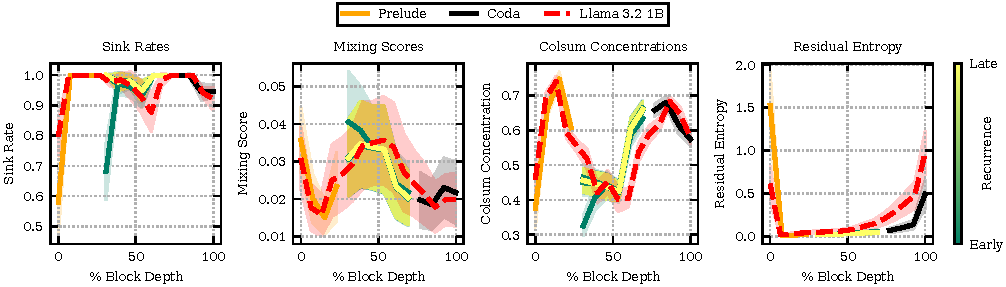
\includegraphics{figures/hellaswag/stages_of_inference/recurrent/Retrofitted_Llama.pdf}
    \caption{\textbf{Stages of inference for each recurrent loop in the retrofitted Llama model \citep{mcleish2025teaching}, run on the HellaSwag dataset.}}
    \label{fig:retrofitted_llama_recurrent_block_stages_hellaswag}
\end{figure}

\begin{figure}[ht]
    \centering    
    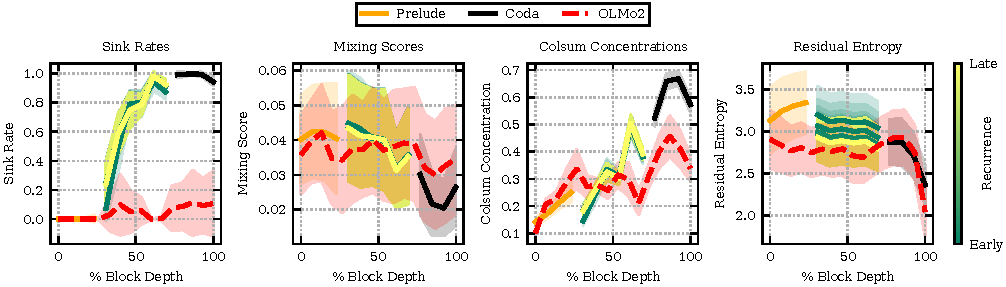
\includegraphics{figures/hellaswag/stages_of_inference/recurrent/Retrofitted_OLMo.pdf}
    \caption{\textbf{Stages of inference for each recurrent loop in the retrofitted OLMo model \citep{mcleish2025teaching}, run on the HellaSwag dataset.} ColSum concentration deviates slightly from its GSM8k counterpart here, but still broadly follows the same stages of inference as the feedforward OLMo model.}
    \label{fig:retrofitted_olmo_recurrent_block_stages_hellaswag}
\end{figure}

\begin{figure}[ht]
    \centering    
    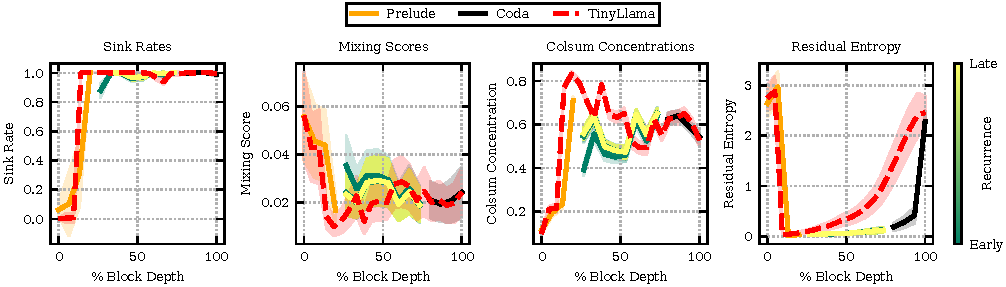
\includegraphics{figures/hellaswag/stages_of_inference/recurrent/Retrofitted_TinyLlama.pdf}
    \caption{\textbf{Stages of inference for each recurrent loop in the retrofitted TinyLlama model \citep{mcleish2025teaching}, run on the HellaSwag dataset.}}
    \label{fig:retrofitted_tinyllama_recurrent_block_stages_hellaswag}
\end{figure}

\FloatBarrier
\subsection{Stability To Unseen Test-Time Recurrences}

This section extends the results presented in \Cref{sec:stability}.

We supplement \Cref{fig:stability_in_total_recurrence} by plotting how stages of inference change per-layer throughout recurrences for additional models: these can be found in \Cref{fig:stages_of_inference_ouro_stability,fig:stages_of_inference_raven_stability,fig:stages_of_inference_retro_llama_stability}. The large standard deviations in \raven{} and retrofitted Llama mixing scores reflect the fact that these models tend to reach different, but still stable, constant states.

\begin{figure}[ht]
    \centering    
    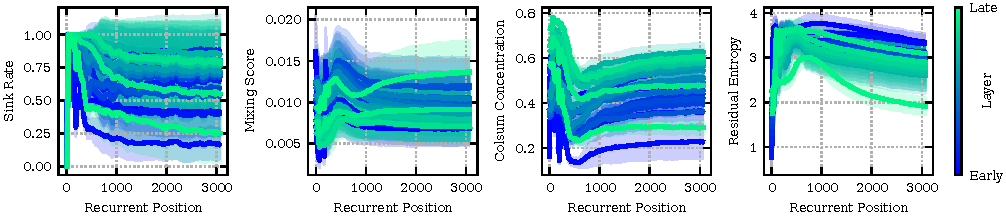
\includegraphics{figures/stages_of_inference/similar_behaviour/Ouro_1.4B_128_steps_means.pdf}
    \caption{\textbf{Stages of inference for each of the distinct blocks in \ouro{} \citep{zhu2025scaling}}, as they are reapplied throughout the model for 128 recurrences. These consistently change throughout the realized depth of the model, reaching no clear fixed point. Mean and standard deviation are over separate inputs to the model, taken over the GSM8k subset.}
    \label{fig:stages_of_inference_ouro_stability}
\end{figure}

\begin{figure}[ht]
    \centering    
    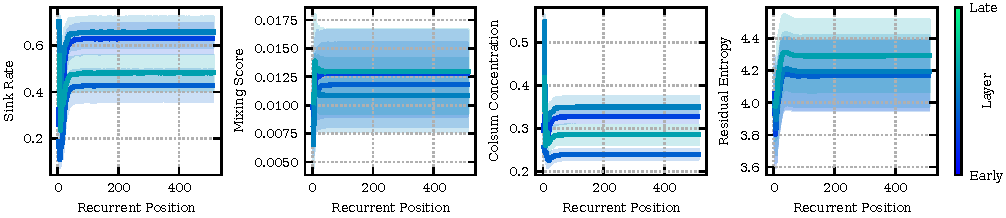
\includegraphics{figures/stages_of_inference/similar_behaviour/Huginn-0125_128_steps_means.pdf}
    \caption{\textbf{Stages of inference for each of the distinct blocks in \raven{} \citep{geiping2025scaling}}, as they are reapplied throughout the model for 128 recurrences. These converge to constant behavior. Mean and standard deviation are over separate inputs to the model, taken over the GSM8k subset.}
    \label{fig:stages_of_inference_raven_stability}
\end{figure}

\begin{figure}[ht]
    \centering    
    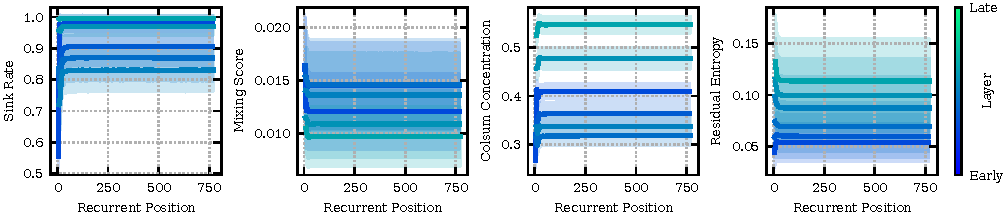
\includegraphics{figures/stages_of_inference/similar_behaviour/Retrofitted_Llama_128_steps_means.pdf}
    \caption{\textbf{Stages of inference for each of the distinct blocks in retrofitted Llama \citep{mcleish2025teaching},} as they are reapplied throughout the model for 128 recurrences. These converge to constant behavior. Mean and standard deviation are over separate inputs to the model, taken over the GSM8k subset.}
    \label{fig:stages_of_inference_retro_llama_stability}
\end{figure}

We additionally plot the extended versions of \Cref{fig:stability_in_percentage_depth} in \Cref{fig:stages_of_inference_ouro_stability_recurrence,fig:stages_of_inference_raven_stability_recurrence,fig:stages_of_inference_retro_llama_stability_recurrence}.

\begin{figure}[ht]
    \centering    
    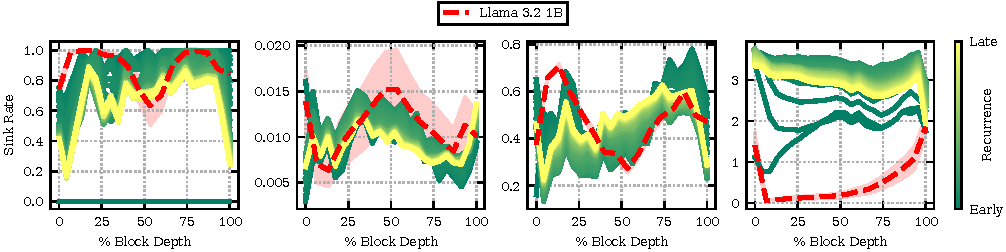
\includegraphics{figures/stages_of_inference/recurrent/Ouro_1.4B_128_steps_to_fixed_point.pdf}
    \caption{\textbf{Stages of inference for \ouro{} with each of 128 recurrences}, visualized over percentage recurrent depth. These consistently change with successive recurrences, deviating significantly from the stages of inference seen with train-time recurrences.}
    \label{fig:stages_of_inference_ouro_stability_recurrence}
\end{figure}

\begin{figure}[ht]
    \centering    
    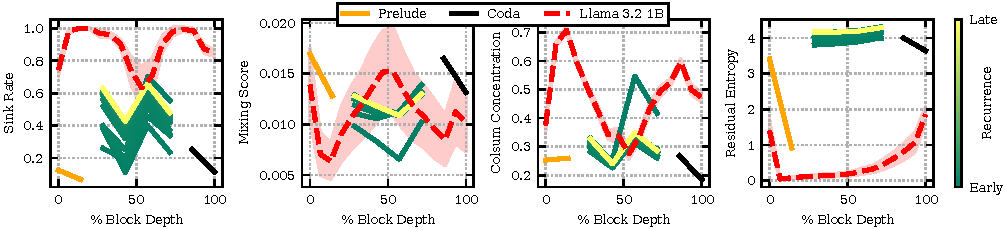
\includegraphics{figures/stages_of_inference/recurrent/Huginn-0125_128_steps_to_fixed_point.pdf}
    \caption{\textbf{Stages of inference for \raven{} with each of 128 recurrences}, visualized over percentage recurrent depth. These quickly reach a fixed point and do not deviate far from their starting stages of inference.}
    \label{fig:stages_of_inference_raven_stability_recurrence}
\end{figure}

\begin{figure}[ht]
    \centering    
    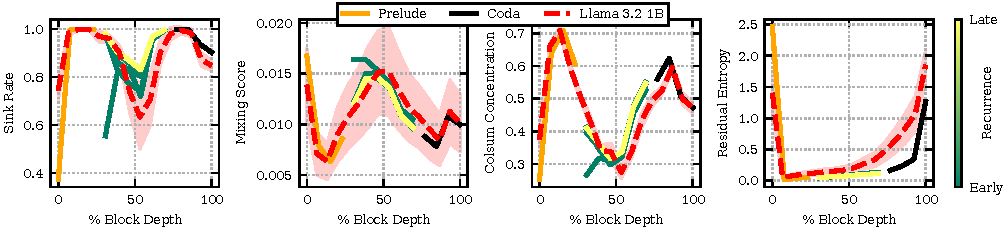
\includegraphics{figures/stages_of_inference/recurrent/Retrofitted_Llama_128_steps_to_fixed_point.pdf}
    \caption{\textbf{Stages of inference for retrofitted Llama with each of 128 recurrences}, visualized over percentage recurrent depth. These quickly reach a fixed point and do not deviate far from their starting stages of inference.}
    \label{fig:stages_of_inference_retro_llama_stability_recurrence}
\end{figure}

\begin{figure}[ht]
    \centering    
    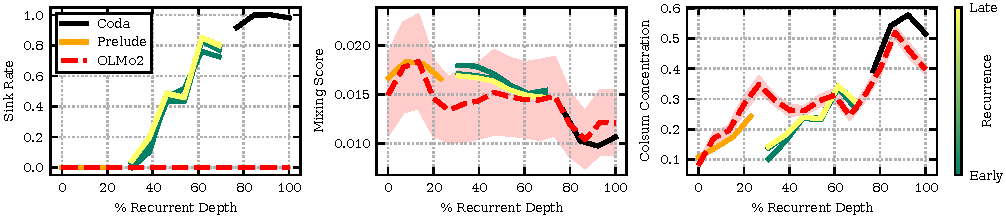
\includegraphics{figures/stages_of_inference/recurrent/Retrofitted_OLMo_128_steps_to_fixed_point.pdf}
    \caption{\textbf{Stages of inference for retrofitted OLMo-2 with each of 128 recurrences}, visualized over percentage recurrent depth. These quickly reach a fixed point and do not deviate far from their starting stages of inference.}
    \label{fig:stages_of_inference_retro_olmo_stability_recurrence}
\end{figure}

\FloatBarrier
\subsection{How Architecture Choices Affect the Formation of Stages of Inference}\label{appen:architecture_stages_of_inference}

Here we present additional results to supplement those in \Cref{sec:self_organising_soi}. The extended stages of inference metrics for the models visualized in \Cref{fig:summary_training_stages_of_interest} are presented in \Cref{fig:r4s,fig:r8s,fig:r12s}. Equivalent models with added input injection are visualized in \Cref{fig:r4si,fig:r8si,fig:r12si}, and equivalent models without sandwich layers in \Cref{fig:r4,fig:r8,fig:r12}.

It appears in these small scale experiments that feedforward stages of inference are most closely replicated without input injection, and using sandwich layers, as in \Cref{fig:r4s,fig:r8s,fig:r12s}. The addition of input injection appears to mean that the \emph{final} recurrence follows the feedforward stages of inference more closely, but to the detriment of earlier recurrences.

\begin{figure}[ht]
    \centering
    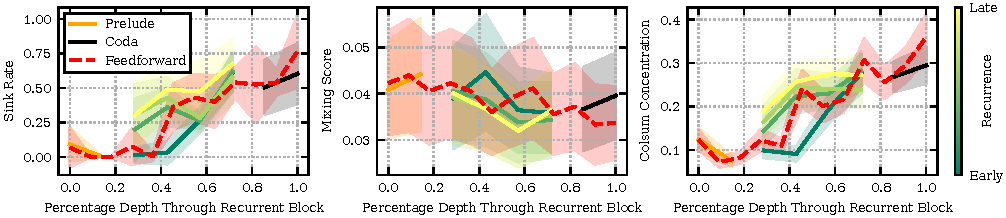
\includegraphics{figures/training/R4S.pdf}
    \caption{\textbf{Stages of inference metrics for a small-scale Looped Transformer of configuration $(2,4 \otimes 4,2)$}, compared to a ``control'' feedforward Transformer with the same training configuration and depth 12.}
    \label{fig:r4s}
\end{figure}

\begin{figure}[ht]
    \centering
    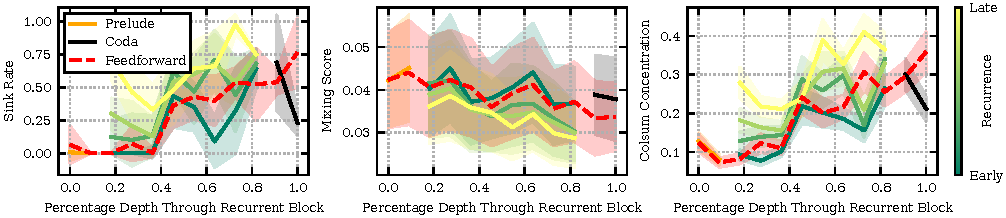
\includegraphics{figures/training/R8S.pdf}
    \caption{\textbf{Stages of inference metrics for a small-scale Looped Transformer of configuration $(2,8 \otimes 4,2)$}, compared to a ``control'' feedforward Transformer with the same training configuration and depth 12.}
    \label{fig:r8s}
\end{figure}

\begin{figure}[ht]
    \centering
    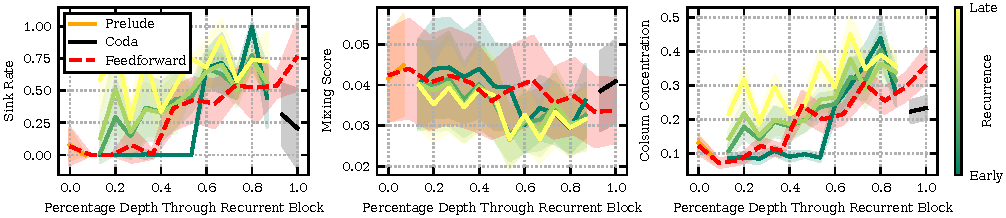
\includegraphics{figures/training/R12S.pdf}
    \caption{\textbf{Stages of inference metrics for a small-scale Looped Transformer of configuration $(2,12 \otimes 4,2)$}, compared to a ``control'' feedforward Transformer with the same training configuration and depth 12.}
    \label{fig:r12s}
\end{figure}

%%%%%%%%

\begin{figure}[ht]
    \centering
    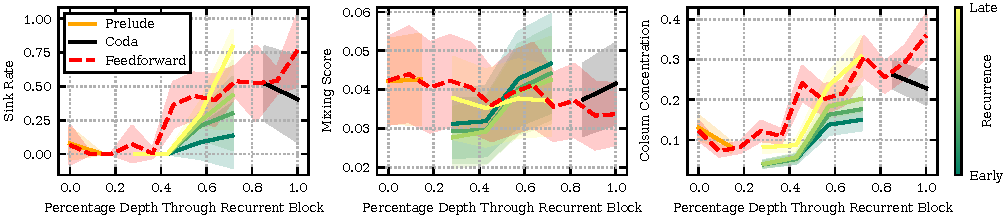
\includegraphics{figures/training/R4SI.pdf}
    \caption{\textbf{Stages of inference metrics for a small-scale Looped Transformer of configuration $(2,4 \otimes 4,2)_I$}, compared to a ``control'' feedforward Transformer with the same training configuration and depth 12.}
    \label{fig:r4si}
\end{figure}

\begin{figure}[ht]
    \centering
    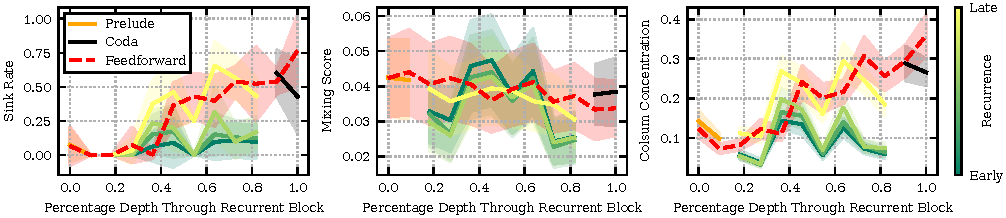
\includegraphics{figures/training/R8SI.pdf}
    \caption{\textbf{Stages of inference metrics for a small-scale Looped Transformer of configuration $(2,8 \otimes 4,2)_I$}, compared to a ``control'' feedforward Transformer with the same training configuration and depth 12.}
    \label{fig:r8si}
\end{figure}

\begin{figure}[ht]
    \centering
    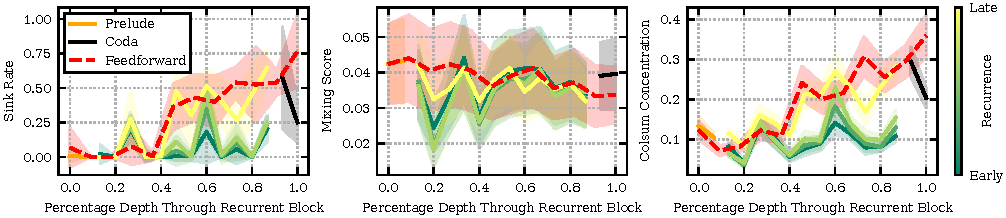
\includegraphics{figures/training/R12SI.pdf}
    \caption{\textbf{Stages of inference metrics for a small-scale Looped Transformer of configuration $(2,12 \otimes 4,2)_I$}, compared to a ``control'' feedforward Transformer with the same training configuration and depth 12.}
    \label{fig:r12si}
\end{figure}

%%%%%%

\begin{figure}[ht]
    \centering
    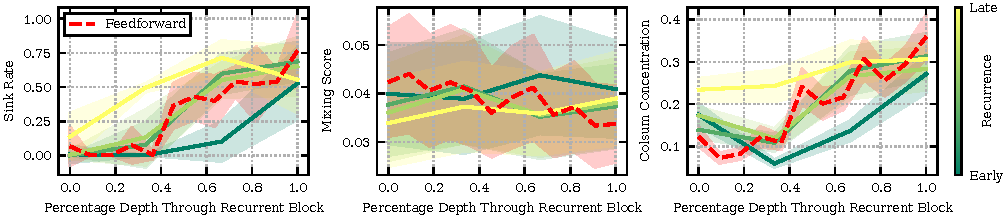
\includegraphics{figures/training/R4.pdf}
    \caption{\textbf{Stages of inference metrics for a small-scale Looped Transformer of configuration $(0,4 \otimes 4,0)$}, compared to a ``control'' feedforward Transformer with the same training configuration and depth 12.}
    \label{fig:r4}
\end{figure}

\begin{figure}[ht]
    \centering
    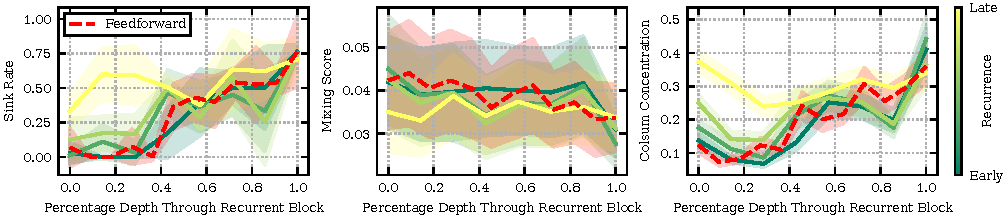
\includegraphics{figures/training/R8.pdf}
    \caption{\textbf{Stages of inference metrics for a small-scale Looped Transformer of configuration $(0,8 \otimes 4,0)$}, compared to a ``control'' feedforward Transformer with the same training configuration and depth 12.}
    \label{fig:r8}
\end{figure}

\begin{figure}[ht]
    \centering
    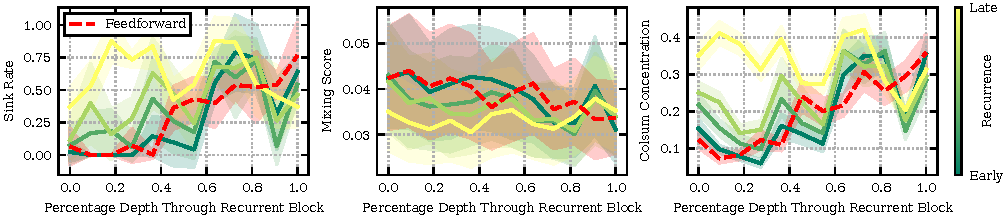
\includegraphics{figures/training/R12.pdf}
    \caption{\textbf{Stages of inference metrics for a small-scale Looped Transformer of configuration $(0,12 \otimes 4,0)$}, compared to a ``control'' feedforward Transformer with the same training configuration and depth 12.}
    \label{fig:r12}
\end{figure}